\documentclass[10pt]{beamer}


\usepackage[utf8]{inputenc}
\usetheme{metropolis}
\usepackage{appendixnumberbeamer}
\usepackage[defaultsans]{droidsans}


\usepackage{tikz}
\usetikzlibrary{positioning}
\usepackage{fancyvrb}
\usepackage{booktabs}
\usepackage[scale=2]{ccicons}

\usepackage{xparse}

\usepackage{xspace}
\newcommand{\themename}{\textbf{\textsc{metropolis}}\xspace}

\usepackage{array}


\title{High Level Assembler Plugin}
%\subtitle{Software project}
\date{Supervisor: Miroslav Kratochvíl}
\author{Michal Bali, Marcel Hruška, Peter Polák, Adam Šmelko, Lucia Tódová}
% \institute{Center for modern beamer themes}
% \titlegraphic{\hfill\includegraphics[height=1.5cm]{logo.pdf}}

\begin{document}

\maketitle


\begin{frame}[standout]{Motivation}
\centering
\hspace*{-1cm}
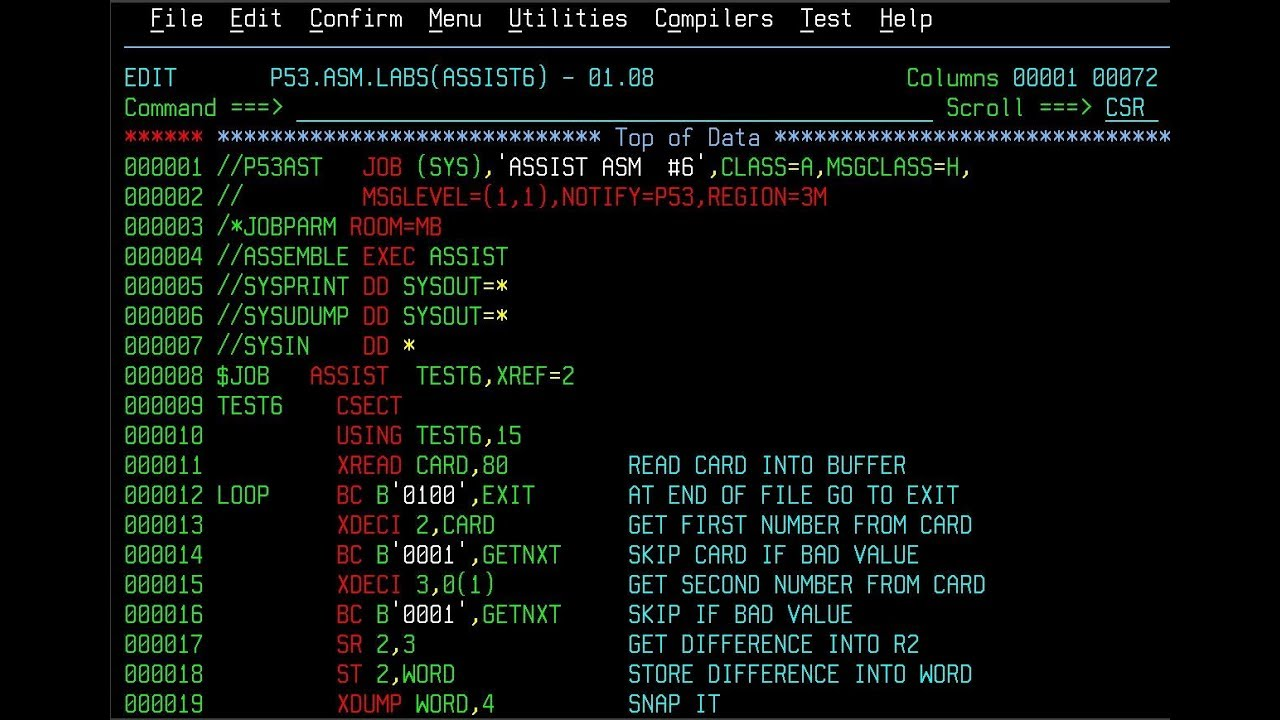
\includegraphics[width=12.6cm]{img/maxresdefault}
\pause
\footnotesize Your Account Balance May Still Rely On Such Code!

\end{frame}

\begin{frame}{Project goals}
    \begin{itemize}
    	\item HLASM support for contemporary source code editors using the Language Server Protocol
    	\item Code validation
    	\item Code navigation (Go to definition, Find all references, \dots)
    	\item Tooltips, autocompletion, \dots
    \end{itemize}

    In the long term:
    \begin{itemize}
        \item Simplify orientation in legacy code
        \item Allow transitioning to some modern language % COBOL
    \end{itemize}
\end{frame}


\begin{frame}{The HLASM language}

There are 3 types of instructions:
\begin{enumerate}
	\item Machine instructions
	\item Assembler instructions \\\quad{\small (`compile'-time variables, modifications of assembler program state)}
	\item Conditional Assembly instructions \\\quad{\small (basically a Turing-complete macro system)}
\end{enumerate}

\textbf{Main problem:} Code interpretation heavily depends on 2.~and 3.

\end{frame}

\newcommand{\aaa}[2]{\alert<#1>{#2}}
\begin{frame}[fragile]{Example --- assembler instructions}
\begin{Verbatim}[commandchars=\\\{\}]
[00]              \aaa{2}{LR    1,2}
[01]              \aaa{3}{DS    CL(LEN)}
[02]   \aaa{4}{ADDR       DS    CL(SIZE)}
[03]   \aaa{5}{HERE       DS    CL5}
[04]
[05]   \aaa{6}{LEN        EQU   HERE-ADDR}
[06]   \aaa{7}{SIZE       EQU   1}
\end{Verbatim}

Output layout:
\begin{center}
\begin{tikzpicture}[node distance=0mm, font=\tt]
\node[rectangle,draw, minimum width=7em, minimum height=2em] (a) {\only<2->{\alert<2>{2}}};
\node[rectangle,draw, minimum width=7em, minimum height=2em, right=of a] (b) {\only<3->{\alert<3>{LEN}}\only<3-5>{=?}\only<6>{=\alert{SIZE}}\only<7>{=\alert{1}}};
\node[rectangle,draw, minimum width=7em, minimum height=2em, right=of b] (c) {\only<4->{\alert<4>{SIZE}}\only<4-6>{=?}\only<7>{=\alert{1}}};
\node[rectangle,draw, minimum width=7em, minimum height=2em, right=of c] (d) {\only<5->{\alert<5>{5}}};

\node[below=of b.south east, minimum width=5em, anchor=east, rotate=90] {\only<4->{ADDR $\to$}};
\node[below=of c.south east, minimum width=5em, anchor=east, rotate=90] {\only<5->{HERE $\to$}};
\end{tikzpicture}
\end{center}

\end{frame}

\begin{frame}[fragile]{Example --- Conditional Assembly}
\begin{Verbatim}[commandchars=\\\{\}]
[00]   &VAR       \aaa{3}{SETA    1}
[01]   .LOOP      ANOP         
[02]   \aaa{2}{SYM&VAR}    DC      C'A'
[03]              \aaa{4}{AIF     (D'SYM3).END}
[04]   \aaa{3}{&VAR       SETA    &VAR+1}
[05]              \aaa{3}{AIF     (&VAR LE 4).LOOP}
[06]   .END       END     
\end{Verbatim}

\pause
\textbf{Output:}
\begin{Verbatim}[commandchars=\\\{\}]
[00]   \aaa{2}{SYM1}       DC      C'A' \pause
[01]   SYM2       DC      C'A'
[02]   \aaa{4}{SYM3}       DC      C'A' \pause
[03]              END
\end{Verbatim}
\end{frame}

\begin{frame}{Architecture}
\centering
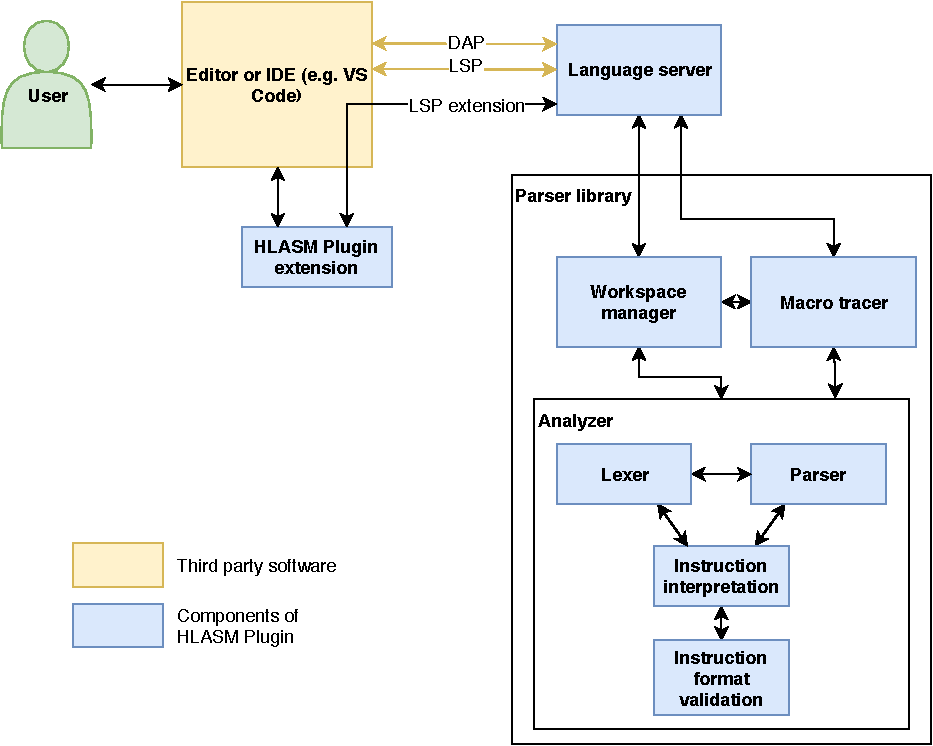
\includegraphics[width=10.5cm]{img/hlasm_architecture}
\end{frame}


\begin{frame}{Already done: Preview version}
\centering
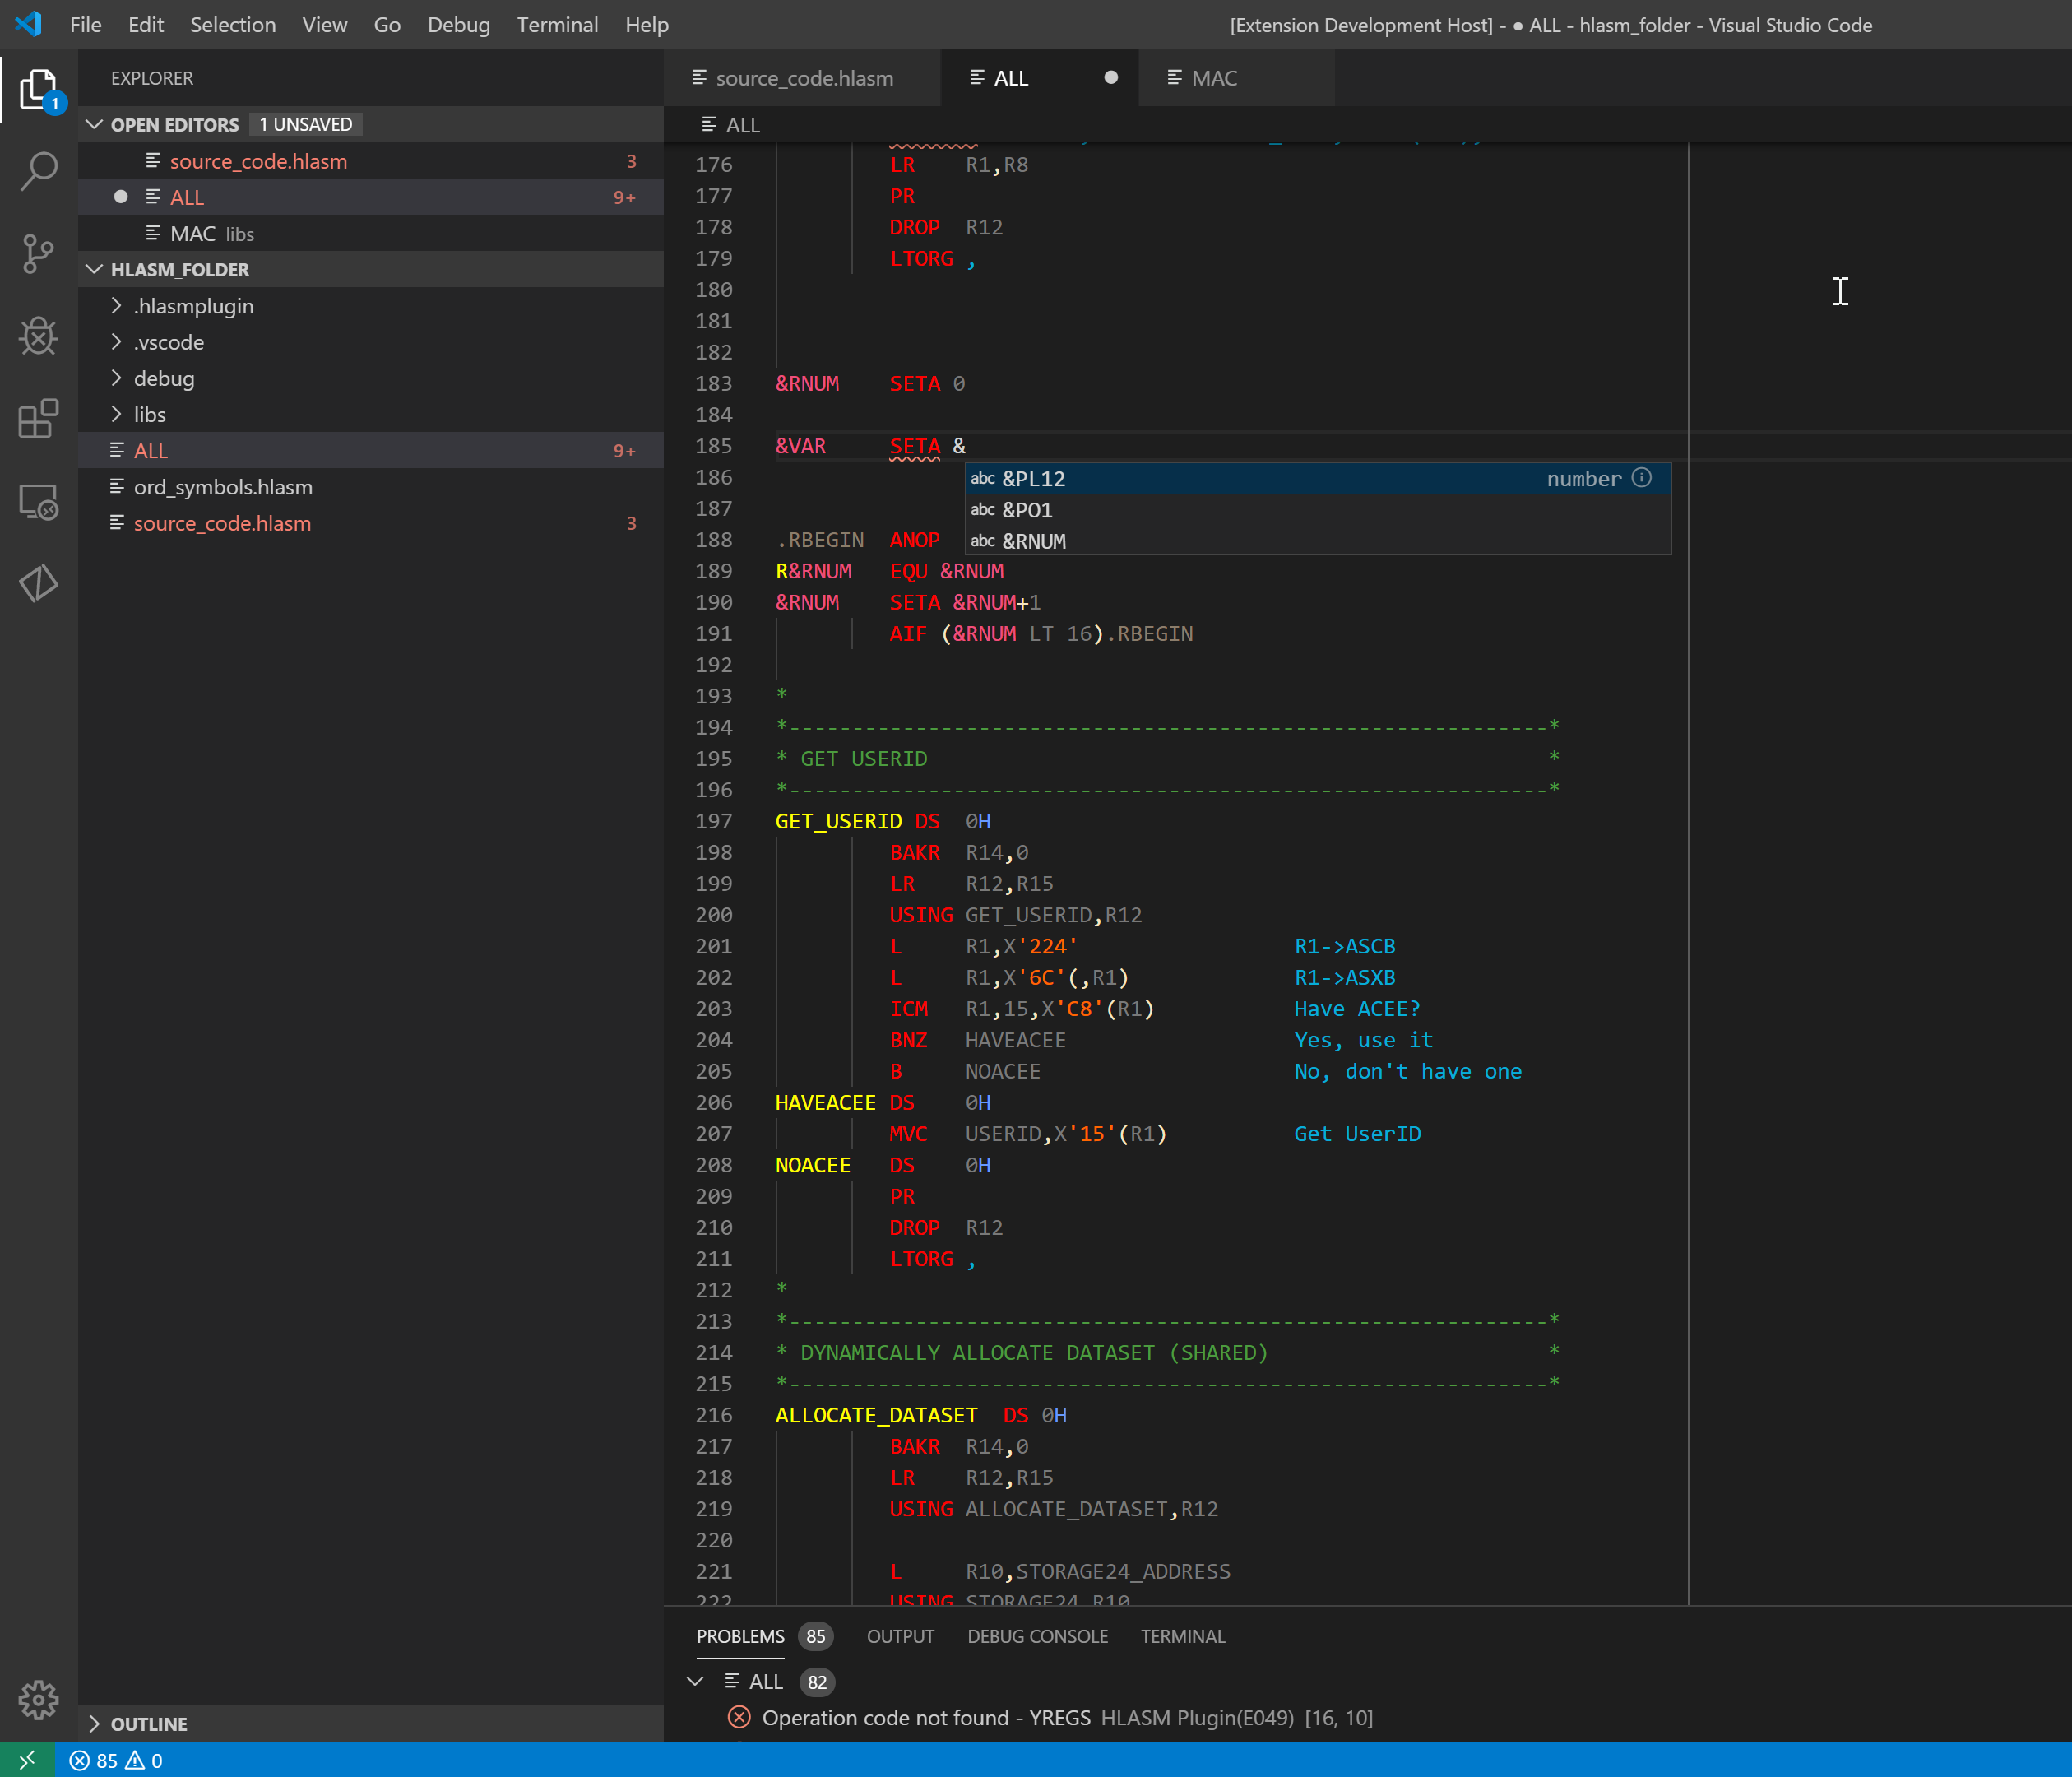
\includegraphics[width=9cm]{img/screenshot}

\footnotesize
Source code taken from \url{https://github.com/zhaimlill/EnhanceStartOnZ}
\end{frame}


\begin{frame}{Current timeline}

\centering
\hspace*{-0.95cm}
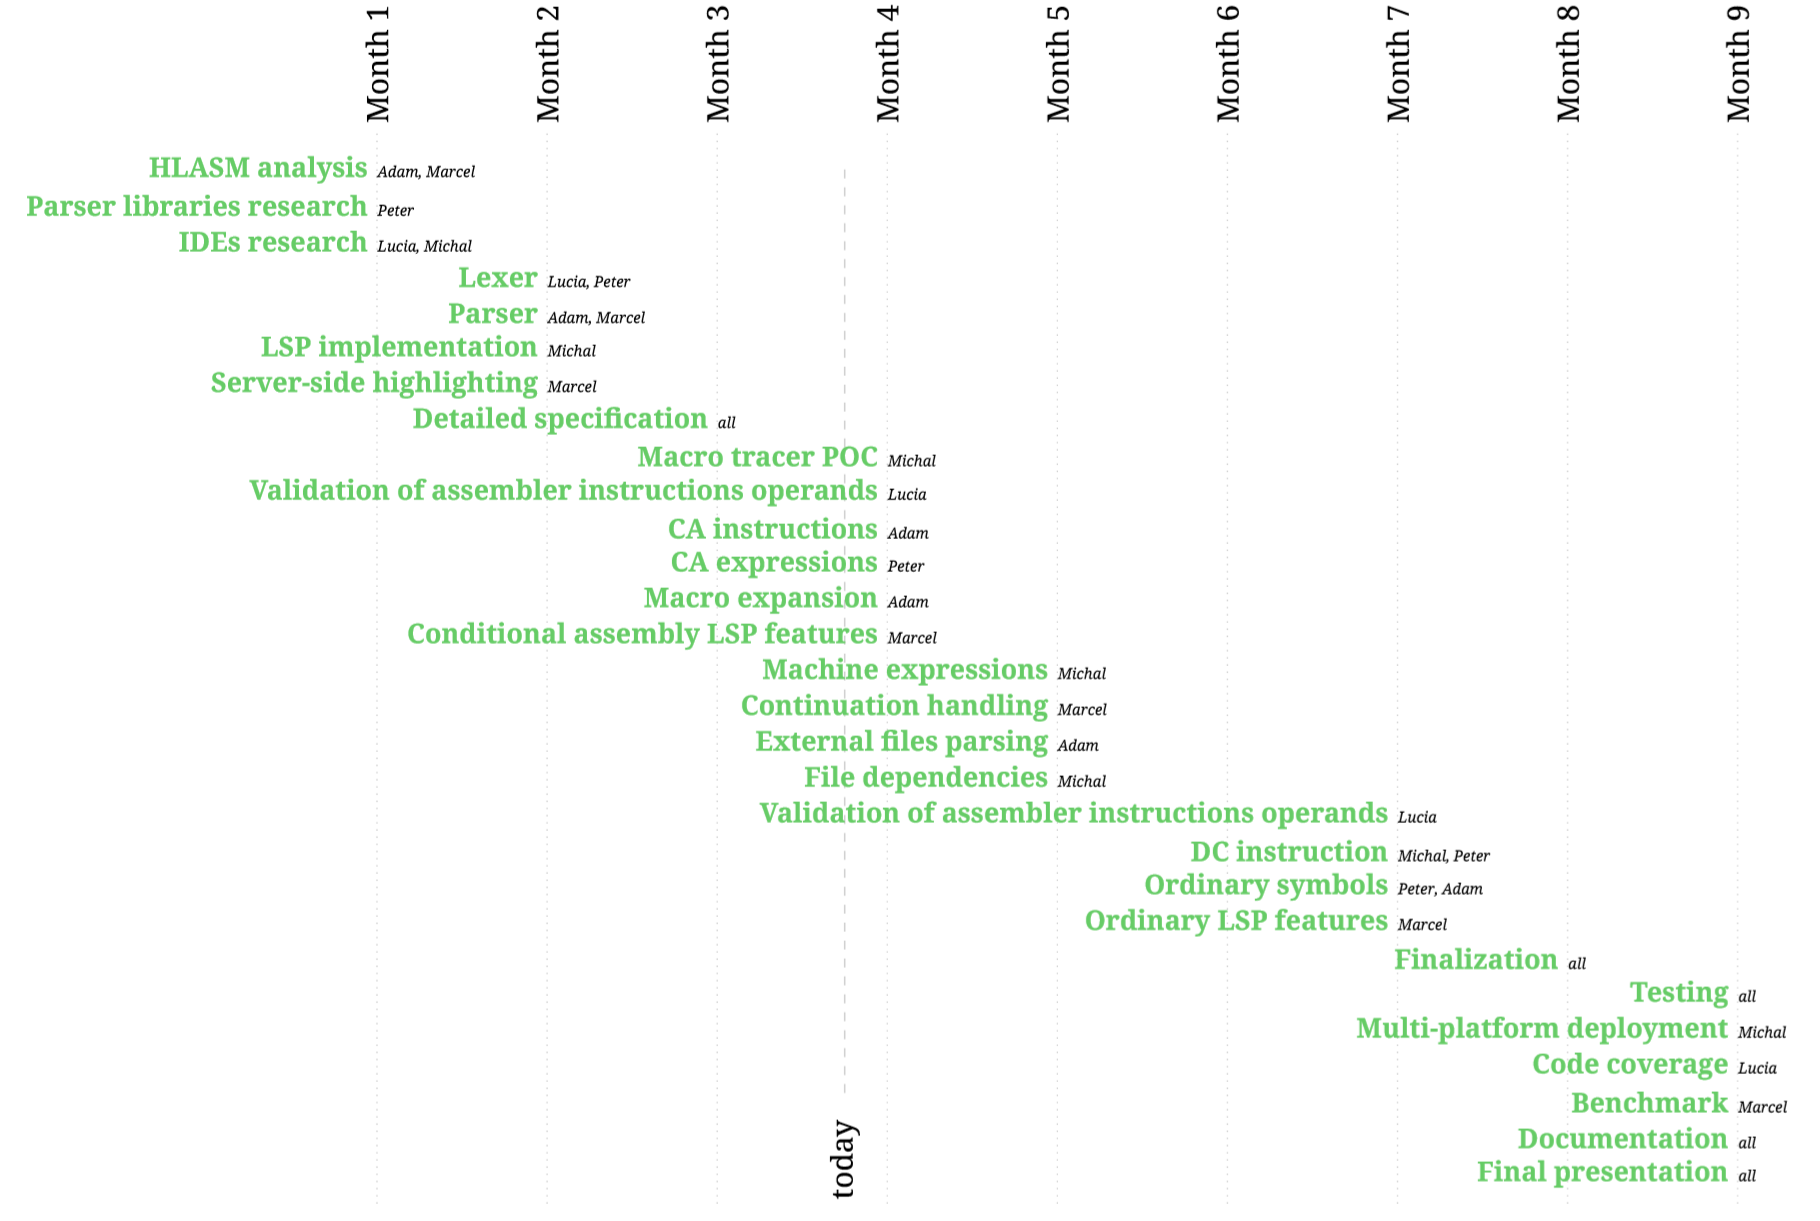
\includegraphics[width=12.5cm]{img/timeline}

\end{frame}


\begin{frame}{Future perspectives}
\begin{itemize}
\item the prototype has been already tested\\ on realistically large projects
	\begin{itemize}
		\item ``proof of concept'' works well
		\item additional integration problems seem unlikely
	\end{itemize}
\item one possible problem:\\ syntax highlighting performance
	\begin{itemize}
		\item small changes require reprocessing\\ of huge amounts of generated code
		\item optimizations are possible
	\end{itemize}
\end{itemize}
\end{frame}


\begin{frame}[standout]
  Thank you for attention.

  \small Questions?
\end{frame}


\end{document}
